\section{案例二：CVE-2025-2241（Hive \texttt{ClusterProvision} 敏感信息泄漏）}

\subsection{漏洞详解与复现}

\textbf{（1）漏洞背景}

Hive 是 Red Hat Multicluster Engine（MCE）与 Advanced Cluster Management（ACM）中的集群生命周期管理组件，常用于在多集群场景下自动化创建与托管 OpenShift/Kubernetes 集群。
在 vSphere 场景中，Hive 需要使用 vCenter 凭据完成集群的基础设施供应与后续管理。

\textbf{CVE 描述}：CVE-2025-2241 指出 Hive 在完成 vSphere 集群供应（provisioning）后，会将 vCenter 凭据暴露在 \texttt{ClusterProvision} 对象中。由于 \texttt{ClusterProvision} 属于自定义资源（CR），拥有其\textbf{读取权限}的用户可直接从该对象中提取敏感凭据，即使该用户并不具备对 Kubernetes \texttt{Secret} 的访问权限。
该问题会导致未授权 vCenter 访问、基础设施与集群管理风险，并可能进一步演化为权限提升。

\textbf{CVSS 信息}：CNA（Red Hat）给出的向量为 \texttt{CVSS:3.1/AV:N/AC:H/PR:L}，基准分 8.2（High）。其含义可理解为：攻击者需要一定前置权限（PR:L）和较高攻击复杂度（AC:H），但一旦满足条件，影响范围跨越安全边界（S:C），并造成高机密性与完整性影响（C:H/I:H）。

\textbf{主要成因分类}：敏感信息泄漏 / 配置与对象生命周期缺陷（“Secret 旁路”：敏感数据出现在可读的 CR 状态字段中）。

\textbf{攻击链条描述}：该漏洞可抽象为“\texttt{Secret} 隔离被 CR 可读性绕过”的链条：
\begin{enumerate}
	\item \textbf{权限前置阶段}：攻击者拥有对 \texttt{ClusterProvision} 的 \texttt{get/list/watch} 权限（通常来自聚合角色 \texttt{view/edit} 或错误的绑定）；
	\item \textbf{数据旁路阶段}：Hive 在供应流程中将 vCenter 凭据写入 \texttt{ClusterProvision}（常见位于 \texttt{status} 字段）；
	\item \textbf{凭据提取阶段}：攻击者通过读取 CR YAML/JSON 直接获得凭据；
	\item \textbf{后续风险阶段}：利用 vCenter 凭据对虚拟化平台执行未授权操作，进而影响集群节点与工作负载，造成横向移动或权限提升。
\end{enumerate}

\begin{figure}[htbp]
	\centering
	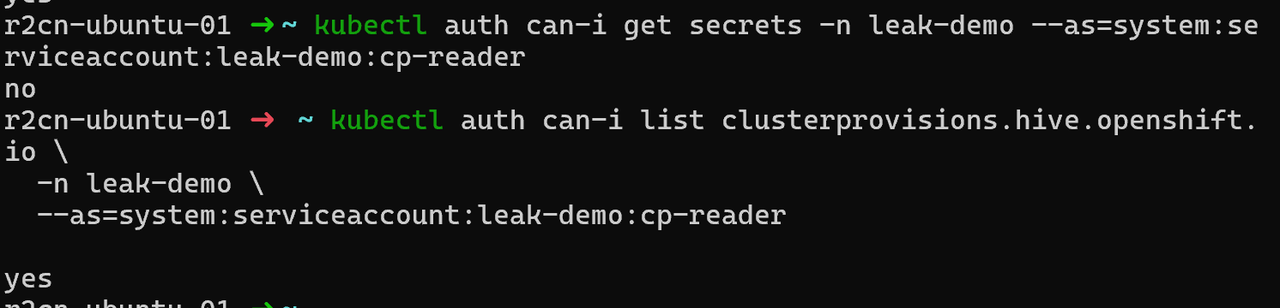
\includegraphics[width=0.95\textwidth]{images/cve2/image.png}
	\caption{CVE-2025-2241：vCenter 凭据通过 \texttt{ClusterProvision} 暴露的风险示意}
	\label{fig:cve-2025-2241-overview}
\end{figure}

\textbf{（2）漏洞复现}

本案例复现目标是验证：\textbf{无 \texttt{Secret} 访问权限但可读 \texttt{ClusterProvision} 的用户}，是否可从对象中提取到 vCenter 凭据。
由于该漏洞涉及敏感凭据泄露，本文仅给出\textbf{受控测试环境}的复现要点，详细 YAML 与命令序列见附录\ref{app:cve-2025-2241}。

\textbf{环境配置}：
\begin{itemize}
	\item 测试集群：OpenShift 或 Kubernetes（部署 ACM/MCE 与 Hive，具体版本以厂商公告与实验环境为准）；
	\item 基础设施：vSphere 环境与可用 vCenter 账号（最小权限、测试专用）；
	\item 权限模型：至少一个“只读用户/角色”，具备 \texttt{ClusterProvision} 读取权限但不具备 \texttt{Secret} 读取权限。
\end{itemize}

\textbf{攻击步骤（摘要）}：
\begin{enumerate}
	\item 创建 vSphere 集群供应配置（Hive \texttt{ClusterDeployment} 等相关对象），触发供应流程；
	\item 使用低权限但可读 \texttt{ClusterProvision} 的身份读取对象并导出 YAML；
	\item 在输出中定位 vCenter 用户名/密码等敏感字段（例如 \texttt{status.vCenter.credentials.*} 或同类结构）。
\end{enumerate}

\textbf{攻击结果}：若在 \texttt{ClusterProvision} 的可读字段中发现明文凭据，则说明“敏感信息通过 CR 状态旁路泄露”成立；该风险不依赖 \texttt{Secret} 读取权限，属于权限边界外泄。

\subsection{策略部署}
使用本文方法生成的最佳安全策略如下（经多智能体评估体系选出）。与“纯升级”不同，本案例强调：\textbf{敏感信息泄漏的治理核心在于读权限面（read surface）与暴露窗口（exposure window）管理}。

\textbf{策略概述}：
\begin{itemize}
	\item \textbf{防控层次（layer）}：身份与权限 / 审计与告警 / 资源生命周期治理 / 准入策略（审计型）
	\item \textbf{防控方法（method）}：RBAC 收敛 + 读取审计与告警 + 供应完成后的对象清理（缩短暴露窗口）+ vCenter 凭据轮换与强化 + “敏感字段守护”检测
	\item \textbf{使用工具}：Kubernetes/OpenShift RBAC、Kubernetes Audit、CronJob/自动化清理、Gatekeeper 或 Kyverno（建议以 \texttt{dryrun/Audit} 方式用于检测）
\end{itemize}

\textbf{策略配置与部署步骤}：为避免正文过长，本案例的复现详细步骤、RBAC 清单、审计策略片段、自动化清理示例与 Gatekeeper/Kyverno 检测规则完整代码见附录\ref{app:cve-2025-2241}。

\subsection{三因素分析}

\textbf{（1）有效性（Effectiveness）}
\begin{itemize}
	\item \textbf{RBAC 收敛}可直接降低“非必要主体读取 \texttt{ClusterProvision}”的概率，是最关键的风险抑制手段；
	\item \textbf{审计与告警}可发现异常读取行为，并在凭据轮换后用于验证风险是否仍存在；
	\item \textbf{对象清理/自动化}可缩短凭据暴露窗口，降低“读取即泄露”的可利用时间；
	\item \textbf{准入策略（审计型）}可帮助在配置漂移或版本回退时及时发现敏感字段再次出现。
\end{itemize}

\textbf{（2）无干扰性（Interference）}
\begin{itemize}
	\item RBAC 收敛主要影响运维/排障可见性，需要通过“按需、限时、可审计”的授权流程替代全局可读；
	\item 审计与告警对业务无直接影响，但会增加日志量与告警治理成本；
	\item 自动化清理需确保不会破坏 Hive 的后续对账/回收流程，建议先在预生产验证并以标签/状态条件精确匹配删除对象。
\end{itemize}

\textbf{（3）可部署性（Deployability）}
\begin{itemize}
	\item RBAC 与审计为平台原生能力，可在多集群场景快速模板化推广；
	\item 清理与轮换为运维流程问题，建议与 GitOps/流水线集成（供应完成后打标签\,$\rightarrow$\,定时清理）；
	\item 准入策略建议从 \texttt{dryrun/Audit} 起步，作为检测与治理辅助，而非强制拦截控制器写入 \texttt{status}（避免影响供应）。
\end{itemize}

